\documentclass[10pt,a4paper]{article}
\usepackage[utf8]{inputenc}
%\usepackage[engl]{babel}
\usepackage[T1]{fontenc}
\usepackage{amsmath}
\usepackage{amsfonts}
\usepackage{amssymb}
\usepackage{graphicx}
\usepackage{bm}
\usepackage[rmargin=1.5cm, lmargin=1.5cm, bmargin=1.5cm]{geometry}
\usepackage{enumitem}
\setitemize{noitemsep,topsep=0pt,parsep=0pt,partopsep=0pt}


\author{Lars Schiller}
\title{Algorithm for predicting the pose of a gecko-inspired soft robot for a given reference input}


\usepackage{multicol}



\begin{document}


\maketitle

Due to the fact that the behaviour of soft materials is difficult to predict with conventional methods, an algorithm based on a geometric optimization problem is presented.
The algorithm can be used to predict the actual pose of the robot for a given reference pose.

\begin{figure}
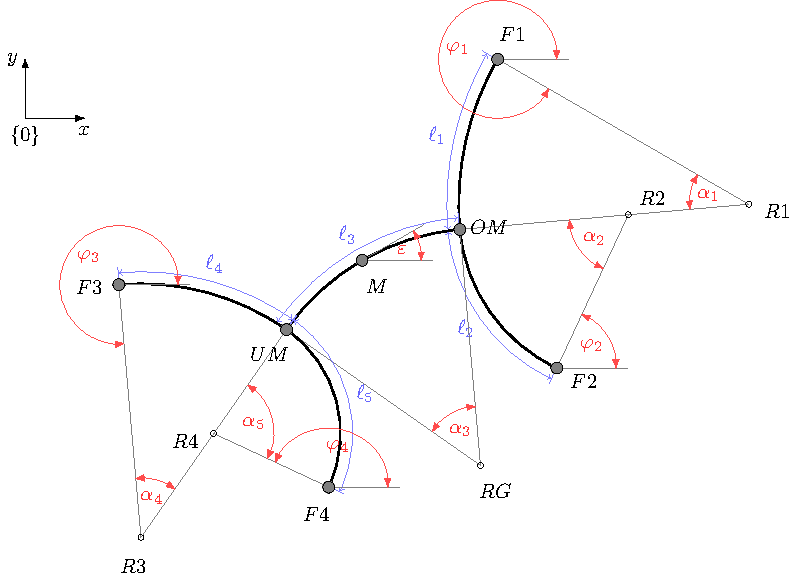
\includegraphics[scale=1]{../Pics/model/model.pdf}
\caption{Nomencalture}
\label{fig:model}
\end{figure}

In order to let the robot take a pose, i.\,e., a position and orientation, the user has nine degrees of freedom at his disposal: the correspondending pressures $p_i$ for the five deformation angles $\alpha_i$ of the limbs $i=1,\dots,5$ and the state of the fixation actuators $f_j \in \{0,1\}$ of the feet $j=1,\dots,4$.
Accordingly, a reference pose can be described by
\begin{equation}
\bm{ref} = \left[ p_1~p_2~p_3~p_4~p_5~f_1~f_2~f_3~f_4~ \right]^\top.
\end{equation}


Mapping function.
\vspace{1cm}

However, this information is not sufficient to describe the robot's actual pose.
%The exact position and orientation of at least one foot must be known.
Experiments have shown that the deformation angle of a limb can vary significantly  at the same pressure level due to the softness of the used material. The length of a limb can also differ.


In order to describe the pose of the robot, the deformation angles $\alpha_i$, the actual lengths of the individual limbs $\ell_i$, and the position and orientation of (at least) one foot ($\bm{r}_{j} \in \mathbb{R}^{2 \times 1}$ and $\varphi_{j}$) must be known (see Fig.~\ref{fig:model}).
For example, if the position and orientation of the front left foot is known, the pose can be described by the following expression:

\begin{equation}
\bm{\alpha} = \left[ \alpha_1~\alpha_2~\alpha_3~\alpha_4~\alpha_5 \right]^\top.
\end{equation}

\begin{equation}
\bm{\ell} = \left[ \ell_1~\ell_2~\ell_3~\ell_4~\ell_5 \right]^\top.
\end{equation}



\begin{equation}
\bm{\rho}_{F_1} = \left[ \alpha_1~\alpha_2~\alpha_3~\alpha_4~\alpha_5 ~\ell_1 ~\ell_2 ~\ell_3 ~\ell_4 ~\ell_5 ~\bm{r}^\top_{1} ~\varphi_1 \right]^\top.
\end{equation}

\begin{equation}
\bm{\rho}_{F_1} = \left[ \bm{x} ~\bm{r}_{1} \right]^\top.
\end{equation}

Here, the pose seems to be independent of the fixed feet. But the dependency lies in the angles of deformation and the actual lengths of the limbs. These must be determined in such a way that the actual positions of the fixed feet correspond to the theoretical positions from the geometric model.
Using the equations \eqref{eq:F1_start}--\eqref{eq:F1_end}, the theoretical positions of all feet can be determined, in case the front left foot is fixed. The equations \eqref{eq:F2_start}--\eqref{eq:F2_end} describe the positions if the front right foot is fixed.
The actual positions of the feet are assumed to be the positions from the previous pose.
This can be used to define the constraint for the new pose.
All newly fixed feet must have the same position as in the previous step:

\newcommand{\mbeq}{\overset{!}{=}}
\begin{equation}
\textnormal{if}~f_i:~~F_{i,j} - F_{i,j-1} \mbeq 0,
\label{eq:constraint}
\end{equation}
where $i$ indicates the individual limbs and $j$ the time sequence.
So, the new pose is strongly dependent on where the newly fixed feet were in the prior pose and what orientation they had.
It has already been mentioned that the lengths and the deformation angles of the limbs are quite variable. 
The orientation angles of the fixation actuators ($c_i$) also have a certain margin.
This can be formulated as a objective function:

\begin{equation}
obj(\bm{x}) = w_{len}\sqrt{\sum_i \left( \ell_{n,i} - \ell_i \right)^2} 
+ w_{ang} \sqrt{\sum_i \left( \varphi_i - \alpha_i \right)^2}
+ w_{ori} \sqrt{\sum_i \textnormal{if}~f_i:~\left( c_{i,j-1} - c_{i, j} \right)^2}
\label{eq:objective_function}
\end{equation}

where the weighting factor $w_{len}$ describes the elasticity of the limbs, $w_{ang}$ the bending stiffness of the limbs and $w_{ori}$ the torsional stiffness of the fixing actuators.
Furthermore, $\ell_{n,i}$ describes the nominal length of the $i$-th limb.
The new actual pose can now be determined by solving the optimization problem:

\begin{equation}
\min_{\bm{x} \in \mathcal{X}} ~ obj(\bm{x})~~ s.\,t.~ \textnormal{if}~f_i:~~F_{i,j} - F_{i,j-1} = 0.
\end{equation}


Here $\bm{x} = \left[ \alpha_1 ~ \beta_1 ~ \gamma ~ \alpha_2 ~ \beta_2 ~ c_1 ~ c_2 ~ \ell_1 ~ \ell_2 ~ \ell_\gamma ~ \ell_3 ~ \ell_4 \right]^T$ describes the variables to be optimized, and $\mathcal{X}$ the set of allowed values.
Each variable has bounds. 
For the deformation angles it is:

.....

Radii:
\begin{equation}
r_i = \frac{360 ~ \ell_i}{2 \pi ~ \varphi_i},~~ \textnormal{for}~ i \in [1,2,\gamma,3,4]
\end{equation}



\clearpage
\begin{multicols}{2}

Coordinates for $F1$ fixed:

\begin{equation}
c_2 = c_1 + \alpha_1 + \beta_1
\label{eq:F1_start}
\end{equation}

\begin{equation}
c_3 = 180 + \gamma + \alpha_2 + c_1 + \alpha_1
\end{equation}

\begin{equation}
c_4 = 180 + \gamma + \alpha_1 - \beta_2 + c_1
\end{equation}


\begin{equation}
R1 =  \begin{bmatrix} 
F1_x +\cos(c_1)~r_1 \\ 
F1_y + \sin(c_1)~r_1\end{bmatrix}
\end{equation}

\begin{equation}
OM =  \begin{bmatrix} 
R1_x - \sin(90-c_1-\alpha_1)~r_1 \\ 
R1_y - \cos(90-c_1-\alpha_1)~r_1 \end{bmatrix}
\end{equation}

\begin{equation}
RG =  \begin{bmatrix} 
OM_x + \cos(90-c_1-\alpha_1)~r_\gamma \\ 
OM_y - \sin(90-c_1-\alpha_1)~r_\gamma \end{bmatrix}
\end{equation}

\begin{equation}
UM =  \begin{bmatrix} 
RG_x - \cos(\gamma - 90 + c_1 + \alpha_1)~r_\gamma \\ 
RG_y - \sin(\gamma - 90 + c_1 + \alpha_1)~r_\gamma \end{bmatrix}
\end{equation}

\begin{equation}
R4 =  \begin{bmatrix} 
UM_x + \sin(\gamma - 90 + c_1 + \alpha_1)~r_4 \\
UM_y - \cos(\gamma - 90 + c_1 + \alpha_1)~r_4 \end{bmatrix}
\end{equation}

\begin{equation}
F4 =  \begin{bmatrix} 
R4_x + \sin(-c_4-90)~r_4 \\
R4_y + \cos(-c_4-90)~r_4 \end{bmatrix}
\end{equation}

\begin{equation}
R3 =  \begin{bmatrix} 
UM_x + \sin(\gamma - 90 + c_1 + \alpha_1)~r_3 \\
UM_y - \cos(\gamma - 90 + c_1 + \alpha_1)~r_3 \end{bmatrix}
\end{equation}

\begin{equation}
F3 =  \begin{bmatrix} 
R3_x - \cos(-c_3)~r_3 \\
R3_y + \sin(-c_3)~r_3 \end{bmatrix}
\end{equation}


\begin{equation}
R2 =  \begin{bmatrix} 
OM_x + \cos(c_1 + \alpha_1)~r_2 \\
OM_y + \sin(c_1 + \alpha_1)~r_2 \end{bmatrix}
\end{equation}

\begin{equation}
F2 =  \begin{bmatrix} 
R2_x + \sin(c_2 - 90)~r_2 \\
R2_y - \cos(c_2 - 90)~r_2 \end{bmatrix}
\label{eq:F1_end}
\end{equation}

\columnbreak


Coordinates for $F2$ fixed:

\begin{equation}
c_1 = c_2 - \alpha_1 - \beta_1
\label{eq:F2_start}
\end{equation}

\begin{equation}
c_3 = 180 + \gamma - \beta_1 + \alpha_2 + c_2
\end{equation}

\begin{equation}
c_4 = 180 + \gamma - \beta_2 + c_2 - \beta_1
\end{equation}


\begin{equation}
R2 = \begin{bmatrix}
F2_x - \sin(c_2 - 90)~r_2 \\
F2_y + \cos(c_2 - 90)~r_2
\end{bmatrix}
\end{equation}

\begin{equation}
OM = \begin{bmatrix}
R2_x - \sin(90- c_2 + \beta_1)~r_2 \\
R2_y - \cos(90- c_2 + \beta_1)~r_2
\end{bmatrix}
\end{equation}

\begin{equation}
RG = \begin{bmatrix}
OM_x + \cos(90- c_2 + \beta_1)~r_\gamma \\
OM_y - \sin(90- c_2 + \beta_1)~r_\gamma
\end{bmatrix}
\end{equation}

\begin{equation}
UM = \begin{bmatrix}
RG_x - \cos(\gamma - 90 + c_2 - \beta_1)~r_\gamma \\
RG_y - \sin(\gamma - 90 + c_2 - \beta_1)~r_\gamma
\end{bmatrix}
\end{equation}

\begin{equation}
R4 = \begin{bmatrix}
UM_x + \sin(\gamma - 90 + c_2 - \beta_1)~r_4 \\
UM_y - \cos(\gamma - 90 + c_2 - \beta_1)~r_4
\end{bmatrix}
\end{equation}

\begin{equation}
F4 = \begin{bmatrix}
R4_x + \sin(-c_4 -90)~r_4 \\
R4_y + \cos(-c_4 -90)~r_4
\end{bmatrix}
\end{equation}

\begin{equation}
R3 = \begin{bmatrix}
UM_x + \sin(\gamma - 90 + c_2 - \beta_1)~r_3 \\
UM_y - \cos(\gamma - 90 + c_2 - \beta_1)~r_3
\end{bmatrix}
\end{equation}

\begin{equation}
F3 = \begin{bmatrix}
R3_x - \cos(-c_3)~r_3 \\
R3_y + \sin(-c_3)~r_3
\end{bmatrix}
\end{equation}


\begin{equation}
R1 = \begin{bmatrix}
OM_x + \sin(90-c_2+\beta_1)~r_1 \\
OM_y + \cos(90-c_2+\beta_1)~r_1
\end{bmatrix}
\end{equation}


\begin{equation}
F1 = \begin{bmatrix}
R1_x - \sin(90-c_1)~r_1 \\
R1_y - \cos(90-c_1)~r_1
\end{bmatrix}
\label{eq:F2_end}
\end{equation}

\end{multicols}




\end{document}